%\documentclass{llncs}
\documentclass{llncs} %[runningheads] for title-header on every page



\typeout{}
\typeout{--------------------------------------------------------------}
\typeout{ +---+ Thesis Template                            }
\typeout{ +---+      Version 2.0, August 2011                         }
\typeout{ +---+  for Instituto Superior Tecnico (IST),                 }
\typeout{ +---+  Universidade T�cnica de Lisboa                         }
\typeout{ * Using Thesis Style form Pedro Tom�s                                }
\typeout{ * Created to write Dissertations                             }
\typeout{ * Conforms with IST Master Degree format and with most important packages setup        }
\typeout{ * Should conform with IST PhD Degree format (not verified)   }
\typeout{                                                              }
\typeout{ AUTHOR: Miguel Amador and Jo�o Marques                                          }
\typeout{                                                              }
\typeout{Important: Use all files in the archive, since this is based in all them. Modify dummy files at wish.                                                              }
\typeout{--------------------------------------------------------------}
\typeout{}

% Defines an additional alphabet... not required in most cases
% ------------------------------------------------------------
% \DeclareMathAlphabet{\mathpzc}{OT1}{pzc}{m}{it}

% PACKAGE babel:
% ---------------
% The 'babel' package may correct some hyphenisation issues of latex. 
% However in most situations it is not required.
\usepackage[english]{babel}

% PACKAGE fontenc:
% -----------------
% chooses T1-fonts and allows correct automatic hyphenation.
%\usepackage[T1]{fontenc}
\usepackage[latin1]{inputenc}
%\usepackage[utf8]{inPUTenc}									% UTF 8, Caracteres ocidentais

% PACKAGE eurosym:
% -----------------
% allows the use of the european currency sign
\usepackage{eurosym}

% PACKAGE lettrine:
% -----------------
% allows the use of drop cap lettering
\usepackage{type1cm}
\usepackage{lettrine}

% Package ulem.
\usepackage{ulem} % Allows the use of other text emphatizer commands
\normalem %defines \emph{} to italic, instead of underline. 
\raggedbottom %declaration makes all pages the height of the text on that page. No extra vertical space is added. The \flushbottom declaration makes all text pages the same height, adding extra vertical space when necessary to fill out the page.

% PACKAGE date time:
% -----------------
% Lets you alter the format of the date that \today returns.
\usepackage{datetime}
\newdateformat{todaythesis}{%
\monthname[\THEMONTH]  \THEYEAR}

% PACKAGE latexsym:
% -----------------
% Defines additional latex symbols. May be required for thesis with many math symbols.
\usepackage{latexsym}

% PACKAGE amsmath, amsthm, amssymb, amsfonts:
% -------------------------------------------
% This package is typically required. Among many other things it adds the possibility
% to put symbols in bold by using \boldsymbol (not \mathbf); defines additional 
% fonts and symbols; adds the \eqref command for citing equations. I prefer the style
% "(x.xx)" for referering to an equation than to use "equation x.xx".
\usepackage{amsmath, amsthm, amssymb, amsfonts, amsbsy}

% PACKAGE multirow, colortbl, longtable:
% ---------------------------------------
% These packages are most useful for advanced tables. The first allows to join rows 
% through the command \multirow which works similarly with the command \multicolumn
% The second package allows to color the table (both foreground and background)
% The third package is only required when tables extend beyond the length of one page;
% with compatibilities with the tabular environment. The last allow the definitions of landscape pages, allowing the use of a different orientation for wider graphics or tables. See package documentation to see the implementation.
\usepackage{multirow}
\usepackage{colortbl}
\usepackage{supertabular}
\usepackage{pdflscape}
% \usepackage{longtable}

% PACKAGE graphics, epsfig, subfigure, caption:
% ---------------------------------------------
% Packages for figures... well you will certainly need these packages, with the exception
% of the 'caption' package. This only allows to define extra caption options.
% Notice that subfigure allows to place figures within figures with its own caption. It
% should be avoided to create an eps file with subfigures. That will mean that you won't be 
% able to reference those subfigures. Instead create an EPS file (the only graphics format supported
% by latex) for each of the subfigures and then use the command \subfigure (see below).
\usepackage{graphics}
\usepackage{graphicx}
\usepackage{epsfig}
\usepackage[hang,small,bf]{subfigure}
%\usepackage[footnotesize,bf,center]{caption}
\usepackage{dcolumn}
\usepackage{bm}
\usepackage{booktabs}
\usepackage{rotating}
\usepackage{multirow}

\usepackage[font=small,labelfont=bf,textfont=normalfont]{caption}

% PACKAGE algorithmic, algorithm
% ------------------------------
% These packages are required if you need to describe an algorithm.
% \usepackage{algorithmic}
% \usepackage[chapter]{algorithm}

% PACKAGE natbib/cite
% -------------------
% The two packages are not compatible, and you should use one of the two. Notice however that the
% IEEE BiBTeX stylesheet is imcompatible with the natbib package. If using the IEEE format, use the 
% cite package instead
%\usepackage[square,numbers,sort&compress]{natbib}
\usepackage{cite}

% PACKAGE acronym
% -----------------
% This package is most useful for acronyms. The package guarantees that all acronyms definitions are 
% given at the first usage. IMPORTANT: do not use acronyms in titles/captions; otherwise the definition 
% will appear on the table of contents.
\usepackage[printonlyused]{acronym}
\usepackage[titletoc,title,header]{appendix}
\usepackage[noauto]{chappg}

% PACKAGE extra_functions
% -----------------
% My Personal package: defines the following commands:
% \fancychapter{chaptername) -> Prints a fancier chapter (you can also use the fancychapter package for this)
% \hline{width} -> use for a replacement of the \hline command
% \Mark1, \Mark2, \Mark3, ...
\usepackage{00.extra_functions}


% PACKAGE hyperref
% -----------------
% Set links for references and citations in document
% Some MiKTeX distributions have faulty PDF creators in which case this package will not work correctly
% Long live Linux :D
\usepackage[plainpages=false]{hyperref}
\hypersetup{
             colorlinks=false,
             citecolor=red,
             breaklinks=true,
             bookmarksnumbered=true,
             bookmarksopen=true,
             pdftitle={Benchmark Kinect},
             pdfauthor={Jo�o Pedro Ribeiro Machado},
             pdfsubject={Master Thesis in Information Systems and Computer Engineering},
             pdfcreator={TeXstudio},
             pdfkeywords={Template, Latex, Thesis}}
\usepackage{float}
%\usepackage[final]{00.listofsymbols}
\usepackage{00.symlist}

% Set paragraph counter to alphanumeric mode
\renewcommand{\theparagraph}{\Alph{paragraph}~--}

\newcommand{\figref}[1]{Figure \ref{#1}}
\newcommand{\equationref}[1]{Equation (\ref{#1})}
\newcommand{\tableref}[1]{Table (\ref{#1})}

\newcommand{\textreg}{$\textsuperscript{\textregistered}$}


% MINE MINE
\newcounter{eqn}
\renewcommand*{\theeqn}{\alph{eqn})}
\newcommand{\num}{\refstepcounter{eqn}\text{\theeqn}\;}

\makeatletter
\newcommand{\putindeepbox}[2][0.7\baselineskip]{{%
    \setbox0=\hbox{#2}%
    \setbox0=\vbox{\noindent\hsize=\wd0\unhbox0}
    \@tempdima=\dp0
    \advance\@tempdima by \ht0
    \advance\@tempdima by -#1\relax
    \dp0=\@tempdima
    \ht0=#1\relax
    \box0
}}
\makeatother


% MINE MINE



% load package with ``framed'' and ``numbered'' option.
\usepackage[framed,numbered,autolinebreaks,useliterate]{mcode}

% something NOT relevant to the usage of the package.
\setlength{\parindent}{0pt}
\setlength{\parskip}{18pt}
\title{\texttt{mcode.sty} Demo}
\author{Florian Knorn, \texttt{florian@knorn.org}}
% //////////////////////////////////////////////////



%% Title
\title{Quantum Pirates} % use \\ if the title is too big
\subtitle{A Quantum Game-Theory Approach to The Pirate Game}

%% Author \inst{1}
\author{Daniela Fontes}
% \thanks{\email{daniela.fontesl@ist.utl.pt}
%% Institute, mails and websites
\institute{	72390\\
		Instituto Superior T\'ecnico
\\
\email{daniela.fontesl@ist.utl.pt}
}



\begin{document}

	\maketitle

	\begin{abstract}
		In this document, we develop a model and a simulation of a quantization scheme for the mathematical puzzle created by Omohundro and Stewart - ``A puzzle for pirates '', also known as Pirate Game. This game is a multi-player version of the game ``Ultimatum '', where the players (Pirates), must distribute fixed number of gold coins acording to some rules.

The Quantum Theory of Games is a field that seeks to introduce the mathematical formalism of Quantum Mechanics in order to explore models of conflict that arise when rational beings make decisions. These models of conflict are pervasive in the structural make-up of our society. The combination of game theory and Quantum Probability, despite not having a practical application, can help in the development of new quantum algorithms. Furthermore the fact that Game Theory is transversal to many areas of knowledge can provide insights to future application of these models.

In this dissertation we focused on the role of quantum entanglement and the use of quantum strategies in the game system. We found that when there is no entanglement the game behaved as the original problem even when the players adopted quantum strategies. When using a unrestricted strategic space and the game system is maximaly entangled we found that the game is strictly determined (like the original problem). We also found that when only a the captain has access to quantum strategies in the Pirate Game, she can obtain all the gold coins. These results corroborate similar findings in the field.

		\keywords Quantum Game Theory; Pirate Game; Quantum Mechanics; Quantum Computing; Game Theory; Probability Theory

\begin{comment}		
{\bf List of Abreviations:}
\begin{acronym}
 

\acro{CPT}[CPT]{Conditional Probability Table}
\acro{DAG}[DAG]{Directed Acyclic Graph} 
\acro{DBN}[DBN]{Dynamic Bayesian Networks}
\acro{HMM}[HMM]{Hidden Markov Models}
\acro{QBN}[QBN]{Quantum Bayesian Networks} 
\end{acronym}
	
\end{comment}
\end{abstract}

\section{Introduction}

% MOTIVACAO

%MOTIVACAO
\subsection{Problem Description}
\label{sec:int_problem}

The Pirate Game is a mathematical, Game Theory, problem; with this work want to explore it in the light of quantum game theory. This means developing a quantization scheme, which is a way to transform the original game in a quantum simulation. Our simulations will be implemented on Matlab.

Despite not having a clear ``real-world'' application yet, modelling games with quantum mechanics rules may aid the development of new algorithms that would be ideally deployed using quantum computers. 

Furthermore applying quantum probabilities to a well established area as Game Theory, which has applications in fields such as Economy, Political Science, Psychology, Biology, might introduce new insights and even relevant practical applications\cite{Eisert2008}. 
\subsection{Contributions and Objectives}
This dissertation contributes to the area of Quantum Game Theory and Quantum Computing. The main contributions expected from this work are:

\begin{itemize}

\item A state of the art and related work research with examples and executable simulations that could be used to facilitate the entry in this field;

\item The design and simulation of an unique Quantum Model, and a comparative study with the original version. The Pirate Game is an example of a mathematical game that has not been modelled in a quantum domain yet;

\item The study of the simulation developed. Specifically to study the role of entanglement, and the quantum strategies.
\end{itemize}
The main objectives with this work are: 

\begin{itemize}
\item To learn how to quantize a classical Game Theory problem;

\item To investigate and compile a set of relevant works on Quantum Models;

\item To compare the Quantum and the Classical versions of a game. Namely to observe how quantum phenomena, such entanglement, and the usage of quantum strategic space may alter the Nash equilibria in a quantum game.

\end{itemize}

%OUTLINE DO DOCUMENTO

%%STUFF IT
\section{Background and Related Work}

\section{Pirate Game}
\label{subsec:description}

The original Pirate Game is a multi-player version of the Ultimatum game that was first published as a mathematical problem in the Scientific American as a mathematical problem posed by Omohundro\cite{Stewart1999}. The main objective of the Pirate Game was to present a fully explainable problem with a non-obvious solution. The problem can be formulated as it follows:

\begin{quotation}
Suppose there are 5 rational pirates: A; B; C; D; E. The pirates have a  loot of 100 indivisible gold coins to divide among themselves.


As the pirates have a strict hierarchy, in which pirate A is the captain and E has the lowest rank, the highest ranking pirate alive will propose a division. Then each pirate will cast a vote on whether or not to accept the proposal. 

If a majority or a tie is reached the goods will be allocated according to the proposal. Otherwise the proposer will be thrown overboard and the next pirate in the hierarchy assumes the place of the captain. 

We consider that each pirate privileges her survival, and then will want to maximize the number of coins received. When the result is indifferent the pirates prefer to throw another pirate overboard and thus climbing in the hierarchy. 
\end{quotation}

\subsection{Analysis of the Pirate Game for $3$ Players}
\label{subsubsec:analysis_PG3players}

In Figure \ref{fig:pg_architecturegametree:extensiveform} we have an extensive form representation of the classic Pirate Game for $3$ players. Each node in the game tree has the number of the player who will make the decision, either to Cooperate (vote yes to the proposal), or Defect. The dashed arrows represent states where the player does not have information of the current state (simultaneous move). 

\begin{figure}[h]
\centering 
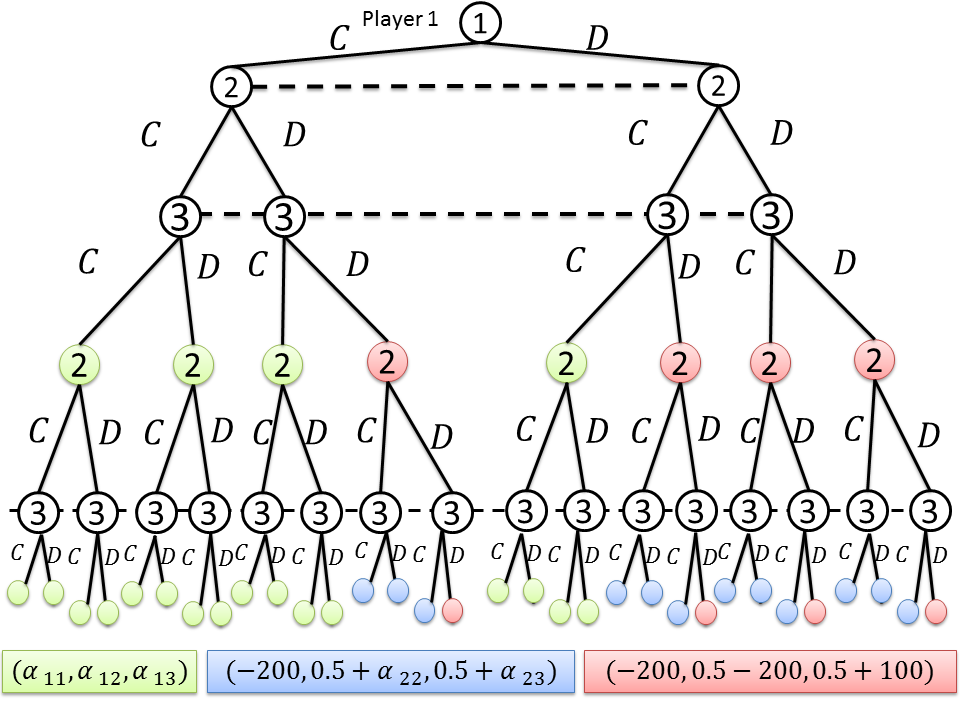
\includegraphics[scale=0.40]{Figures/1.5qubit/FigurasRevistas/Slide1.png}
\caption{Extensive form representation of the classic Pirate Game for $3$ players. }
\label{fig:pg_architecturegametree:extensiveform}
\end{figure}

The green accent, in Figure \ref{fig:pg_architecturegametree:extensiveform}, shown in the nodes represent a state where the first captain (player $1$), will see her proposal accepted, the utility associated . The blue accent denotes the outcomes where the second captain makes a proposal and has seen it accepted. The red accent color represents the outcomes where the player $3$ will be the remaining pirate.

The number of coins will translate directly the utility associated with getting those coins. For example if a pirate receives 5 gold coins and the proposal is accepted he will get a utility of 5. The highest ranking pirate in the hierarchy is responsible to make a proposal to divide the 100 gold coins. This proposal means choosing the number of coins each player gets if the proposal is accepted. A captain $i$ chooses the amount of coins a player $j$ get; this amount will be represented by $\alpha_{ij}$.

In the initial stage of the game the captain will define $\alpha_{11}, \alpha_{12}, \alpha_{13}$, and they will obey to the Equation \ref{eq:goodss}, that imposes the rule that the captain $i$ must allocate all the 100 coins, to the players that are still alive. $N$ the number of pirates in the game. 

\begin{equation}
\label{eq:goodss}
\forall i \in \{1 , 2, ..., N-1\} : \sum_{j=i}^{N}\alpha_{ij}=100, \forall i,j :\alpha_{ij}\in\mathbb{N}_{0}
\end{equation}

The values for $(\alpha_{11}, \alpha_{12}, \alpha_{13})=(99, 0, 1)$ will be the allocation that results in an equilibrium for the $3$ player game .

The proposed goods allocation will be executed if there is a majority (or a tie), in the voting step. A step in the game consists on the highest ranking pirate defining a proposal and the subsequent vote, where all players choose simultaneously an operator. 

If the proposal is rejected the captain will be thrown off board, to account for the fact that this situation is very undesirable for the captain he will receive a negative payoff of $-200$ (that can be seen in the blue and red outcome in Figure \ref{fig:pg_architecturegametree:extensiveform}). This value was derived from the fact that a pirate values her integrity more than any number of coins she might receive.


\begin{quotation}
``When the result is indifferent the pirates prefer to throw another pirate overboard and thus climbing in the hierarchy.''
\end{quotation}

This means that the pirates have a small incentive to climb the hierarchy. For example in the three player classical game, the third player, who has the lowest rank, will prefer to defect the initial proposal if the player 1 doesn't give her a coin, even knowing that in the second round the player 2 will be able to keep the 100 coins. We will account for this preference by assigning an expected value of half a coin ($0.5$), to the payoff of the players that will climb on the hierarchy if the voting fails. This tie breaker is shown in the blue and red outcomes in Figure \ref{fig:pg_architecturegametree:extensiveform}.

\section{Quantum Model}

\section{Analysis}

\section{Simulation}

%%STUFF IT

\section{Conclusion}


\subsection{Future Work}
The principles of quantum computing provide an extremely rich source of ideas to extend other fields of knowledge.
Some suggestions for possible extensions for this work would be:

\begin{enumerate}

\item \textbf{To make conditional measurements by applying the L\"{u}der's Rule} The objective would be to separate each stage of the game with a measurement operation. After a stage where the players made their strategic moves, the resulting quantum state would be de-entangled, projected in order to separate  the sub-game where the vigent proposal was accepted and the complementary state where the proposal was not accepted. The game would be then re-entangled with a new entanglement coefficient. 

\item \textbf{Optimize this Quantum Pirate Game Model.} To model this game as a Quantum Bayesian Network. The Bayesian Networks (also referred to as Belief Networks, Probabilistic networks or causal networks) consist of an Directed Acyclic Graph to represent a set of conditional dependencies between random variables, that provide a compact description that allows to calculate a joint probability distribution, having in mind those dependencies into account. \cite{Tucci2012} proposes a model for Quantum Bayesian Networks, so designing a Quantum Bayesian Network approximation for the Quantum Pirate Game, having the description of this model as a starting point, could be a relevant research topic.

\item \textbf{To implement and test this quantum model with human subjects.} The field of Quantum Cognition tries to explain the Human reasoning process by using principles from quantum game theory, namely quantum probabilities. To expose subjects to a quantum model and having them try to take advantage of the rules of the system might provide valuable insights to the way we reason. 

\item \textbf{Increase the number of players.} Studying the quantum system with $8$ players and $1$ gold coin, would be an interesting extensions for this work. This would allow to experiment the bizarre survival situations that happens when there are not enough coins for the captain to bribe the other pirates. However this particular case of the pirate game would need a $35$-qubit system in order to be studied ($8$ qubits for the first stage, $7$ for the second stage, until reaching a $2$-player sub-game). In a classical computer and full joint probability this would mean working with vectors in the scale $10^{10}$.

\item \textbf{A graphical user interface (GUI) for the Pirate Game.} This would provide a more approachable way to tweak parameters.

\item \textbf{To create and structure a platform to promote scientific dissemination of quantum computing.} While investigating and developing this solution, there was often the thought that it would be important for undergraduate Computer Science students to come with contact with this paradigm. This field is still shrouded with mystery to many people, and this makes it a priority topic for scientific divulgation. In this work we tried to present examples that someone with a basic understanding of Algebra may be able to follow.
\end{enumerate}

 
 






%\bibliographystyle{IEEEtran}
\bibliographystyle{splncs}
%\bibliographystyle{ieeetr}
\bibliography{02.biblio}



\end{document}
